\documentclass{article}\usepackage{amsmath,amsfonts,amssymb}
\usepackage[utf8]{inputenc}
\usepackage{polski}
\usepackage[polish]{babel}
\usepackage[T1]{fontenc}
\usepackage[dvips]{graphicx}
\usepackage{natbib}
\usepackage{setspace}
\usepackage{graphicx}
\usepackage{xcolor}
\usepackage{enumerate}
\usepackage{fancyhdr}
\usepackage{mathtools}
\usepackage{extarrows}
\usepackage{relsize}
\usepackage[hmargin=2cm, vmargin=2cm, hcentering]{geometry}
\usepackage{subfig}
\usepackage{tocloft}
\usepackage{arydshln} % \hdashline
\usepackage[table]{xcolor}
\usepackage[table, dvipsnames]{xcolor}
\usepackage{booktabs}% http://ctan.org/pkg/booktabs
\newcommand{\tabitem}{~~\llap{\textbullet}~~}
\usepackage{enumitem}
\usepackage{caption}
\usepackage{listings}

% \usepackage{tocstyle}
% \usetocstyle{standard}
% \settocfeature{raggedhook}{\raggedright}

\newlist{todolist}{itemize}{2}
\setlist[todolist]{label=}
% \renewcommand\labelitemi{$\square$}

\usepackage{hyperref}
% \hypersetup{
%     colorlinks,
%     citecolor=black,
%     filecolor=black,
%     linkcolor=black,
%     urlcolor=black
% }
% \pagestyle{fancy}
% \fancyhf{}
\doublespacing

\title{Metoda Crouta \\}
\author{Michał Piasecki gr 1. }


\begin{document}

\maketitle

\section{Temat i treść zadania}
W poniższej pracy zajmiemy się problemem rozkładania macierz na postać Crouta: \[ A = L * U   \]. Następnie zajmiemy się rozwiązaniem równań \[  A*X = B     \Leftrightarrow     (LU)*X = B   \]
\boldmath
$A$ - macierz rozmiaru $n \times n $  \\
$L$ - macierz trójkątna dolna rozmiaru $n \times n $  \\
$U$ - macierz trójkątna górna rozmiaru $n \times n$ \\
$B$ - macierz  rozmiaru $n \times m$ \\
$X$ - macierz rozwiązań rozmiaru $n \times m$ \\
\unboldmath
Dodatkowo dla naszych rozkładów będziemy badać niżej wymienionie współczynniki: \\
\begin{itemize}
    \item wskaźnik uwarunkowania macierzy \[ cond(A) =  \|A^{-1} \| \| A \| \]
    \item błąd rozkładu \[ e_{dec} = \frac{\| A - LU \|}{A} \]
    \item współczynnik stabilności \[ wsp_{stab} = \frac{\| x - z \|}{cond(A) \|z\|} \]
    gdzie: \\
    $x$ - dokładne rozwiązanie układu $Ax = b$ \\
    $z$ - rozwiązanie tego samego równania przy pomocy rozkładu Crouta \\
    \item współczynnik poprawności \[ wsp_{pop} = \frac{\| b - Ax \|}{\|A\| \|x\|} \]
    gdzie: \\
    $x$ - rozwiązanie równania przy pomocy rozkładu Crouta
    
    
    
    
\end{itemize}
\\


\newpage
\section{Metoda rozkładu Crouta}
Rozkład Crouta polega na rozłożeniu macierzy $A$ na iloczyn dwóch macierzy $L$ i $U$, gdzie macierz $L$ jest macierzą trójkątną dolną
, a macierz $U$ jest macierzą trójkątną górną, w której elementy na głównej przekątnej równe są 1. \\ 
\[ A = L \times U \]
\\
\begin{equation}
\begin{pmatrix}
  a_{1,1} & a_{1,2} &  a_{1,3} \\
  a_{2,1} & a_{2,2} &  a_{2,3} \\
  a_{3,1} & a_{3,2} & a_{3,3} 
 \end{pmatrix} \\ 
  =  \begin{pmatrix}
  l_{1,1} & 0 &  0 \\
  l_{2,1} & l_{2,2} &  0 \\
  l_{3,1} & l_{3,2} & l_{3,3} 
 \end{pmatrix} \times
 \begin{pmatrix}
  1 & u_{1,2} &  u_{1,3} \\
  0 & 1 &  u_{2,3} \\
  0 & 0 & 1 
\end{pmatrix}
\end{equation}


Zasadnym pytaniem na początku jest czy każdą macierz można sprowadzić do takiej postaci. Okazuje się, że 
\[ \exists_{L,U}{A = L \times U} \Leftrightarrow \forall_{i = 1,2,...,n-1} det(\widetilde{{A}_{i,i}}) \neq 0 \]
gdzie  \[det(\widetilde{{A}_{i,i}})\] to podmacierz A utworzona tylko z pierwszych i-wierszy oraz i-kolumn


Gdy upewnimy się, że powyższy warunek jest spełniony, możemy zacząć rozkład Crouta dla macierz A. Polega on na przyrównywaniu poszczególnych elementów macierzy A do iloczynu macierzy L i U. Dzięki temu, że macierze L i U są trójkątne algorytm wyznaczania takowych macierzy jest dosyć prosty i opiera się na metodach "forward substitution" i "backward substition"  \\

No dobrze, przekształciliśmy naszą macierz do postaci Crouta, ale czemu takowa postać miałaby służyć? Jednym z zastosowań takiej postaci jest względnie szybka możliwośc rozwiązywania układów równań liniowych. Dzięki temu, że nasze macierze są trójkątne wyznaczenie rozwiązań równania jest szybkie i znów opiera się na "forward substitution" i "backward substition".
\[ LU \times X = b \]
Podstawiamy i rozwiązujemy:
\[ UX = Y  \]
\[ LY = b  \]
\[ UX = Y  \]


\newpage
\section{Najważniejsze funkcje}
W tej sekcji zostały zamieszczone dwa najważniejsze programy: rozkład Crouta macierzy A oraz rozwiązanie układu równań 

\lstset{language=Matlab,%
    %basicstyle=\color{red},
    breaklines=true,%
    morekeywords={matlab2tikz},
    keywordstyle=\color{blue},%
    morekeywords=[2]{1}, keywordstyle=[2]{\color{black}},
    identifierstyle=\color{black},%
    stringstyle=\color{mylilas},
    commentstyle=\color{mygreen},%
    showstringspaces=false,%without this there will be a symbol in the places where there is a space
    numbers=left,%
    numberstyle={\tiny \color{black}},% size of the numbers
    numbersep=9pt, % this defines how far the numbers are from the text
    emph=[1]{for,end,break},emphstyle=[1]\color{red}, %some words to emphasise
    %emph=[2]{word1,word2}, emphstyle=[2]{style},    
}
\lstinputlisting{CroutLU.m}
\lstset{language=Matlab,%
    %basicstyle=\color{red},
    breaklines=true,%
    morekeywords={matlab2tikz},
    keywordstyle=\color{blue},%
    morekeywords=[2]{1}, keywordstyle=[2]{\color{black}},
    identifierstyle=\color{black},%
    stringstyle=\color{mylilas},
    commentstyle=\color{mygreen},%
    showstringspaces=false,%without this there will be a symbol in the places where there is a space
    numbers=left,%
    numberstyle={\tiny \color{black}},% size of the numbers
    numbersep=9pt, % this defines how far the numbers are from the text
    emph=[1]{for,end,break},emphstyle=[1]\color{red}, %some words to emphasise
    %emph=[2]{word1,word2}, emphstyle=[2]{style},    
}
\lstinputlisting{solve_linear_equation.m}

\section{Przykłady obliczeniowe}
Zacznijmy od macierzy
\[ A = 
\begin{pmatrix}
  1 & 7 &  3 \\
  10 & 12 &  3 \\
  3 & 5 & 4 
 \end{pmatrix}
 \]

 Po rozkładzie otrzymujemy 
     

\begin{equation}
A = LU = 
\begin{pmatrix}
  1 & 0 &  0 \\
  10 & -58 &  0 \\
  3 & -16 & 2.4483 
 \end{pmatrix} 
 \begin{pmatrix}
  1 & 7 &  3 \\
  10 & 1 &  0.4655 \\
  3 & -16 & 1 
 \end{pmatrix} 
 
 \end{equation}
 Okazuje się, że 
 \[e_{dec}(A) = 0 \]
 Co oznacza, że nasz algorytm przekształcił macierz  do postaci Crouta bez żadnego błędu tzn.
 \[ A = LU\]
 Czy nasz algorytm przekształci idealnie dowolną macierz? Niestety nie :( \\
 Weźmy macierz 
 
 \begin{equation}
C =  
\begin{pmatrix}
  88.52 & 683.71 &  110,35 \\
  798.35 & 132.03 &  117.49 \\
  943 & 722.72 & 640.71 
 \end{pmatrix} 
 \end{equation}
 Okazuje się, że tutaj:
  \[e_{dec}(B) = 3.42 \times 10^{-13} \]
 Nasza macierz została przekształcona z błędem, ale bardzo małym.
 
 Warto byłoby dowiedzieć się jak często dla macierzy $A$, bedzięmy mieli:
   \[e_{dec}(A) = 0 \]
 Niech $X$ będzie zmienną losową przyporządkowującej macierzy jej błąd rozładu. Po kilkukrotnym wygenerowaniu 1000 dowolnych macierzy o wymiarach  $3 \times 3$ okazało się 
 \[ P(X = 0) \approx \frac{1}{4} \]
 Zobaczmy jeszcze wygląda dystrybuanta z takich danych:
 \begin{center}
   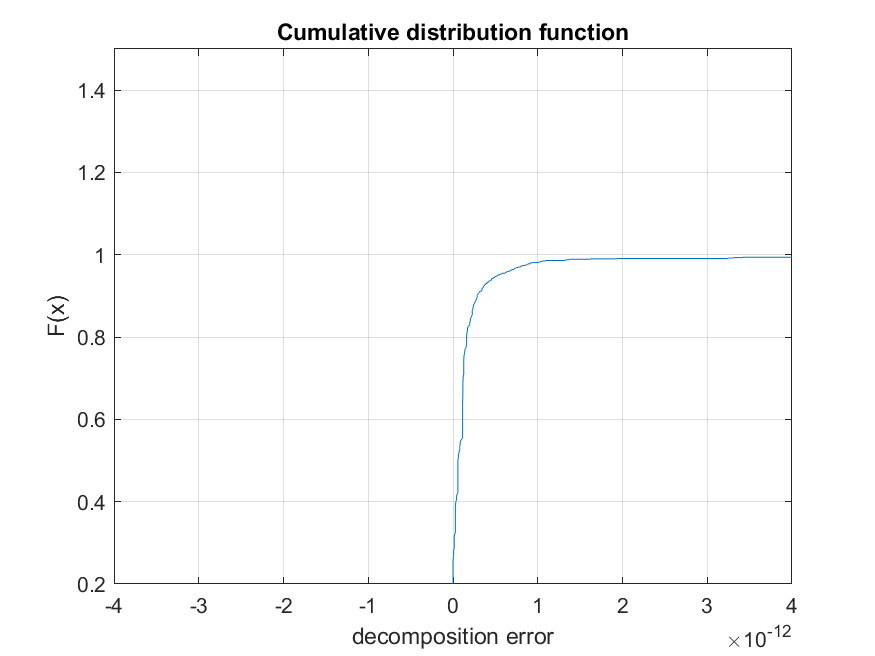
\includegraphics[scale=1]{Cumulative_distribution.png}
\end{center}
Z wykresu łatwo możemy odczytać że prawdopodobieństwo, że 
\[P(X <10^{-12}) > 0.9\] 
co jest całkiem miła informacją - błędy jakie generuje nasz rozkład są bardzo niewielkie.

Pytanie co się dzieje w przypadku macierzy o większych rozmiarach? Ponownie utworzyliśmy 1000 dowolnych macierzy o rozmiarach kolejno: $4 \times 4$, $10 \times 10$,$20 \times 20$
Otrzymujemy następujące wykresy:
 \begin{center}
   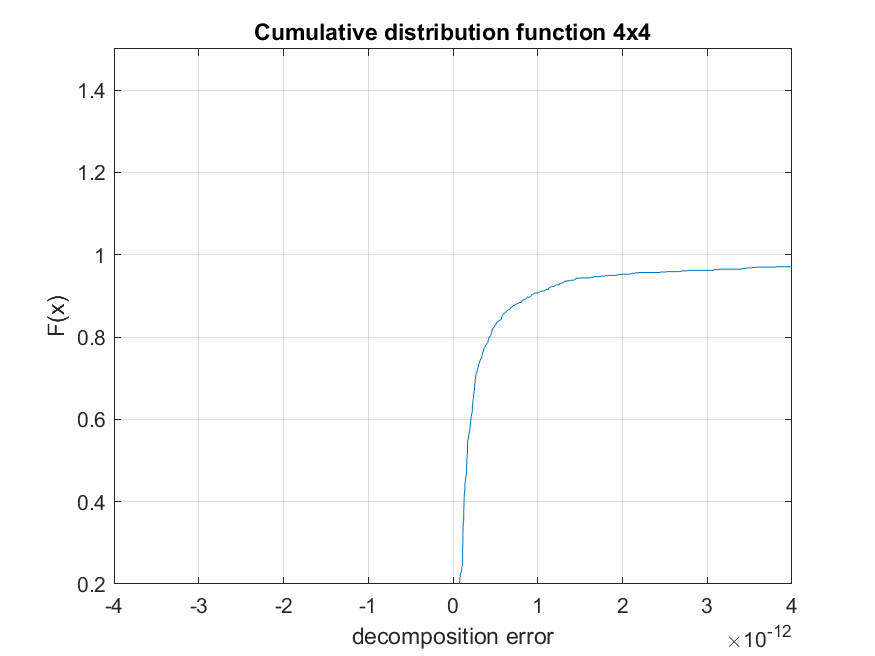
\includegraphics[scale=1]{4x4.png}
\end{center}
 \begin{center}
   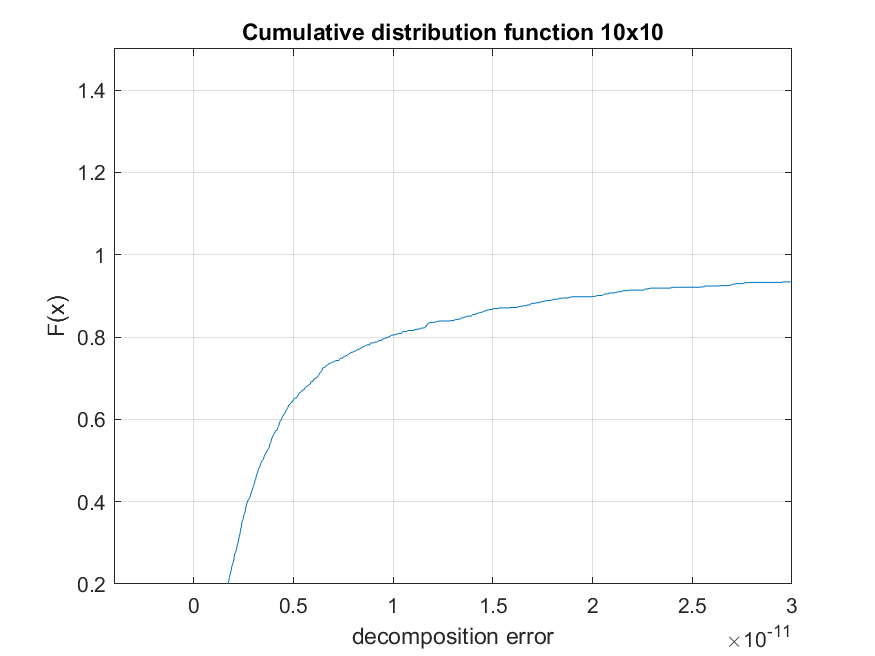
\includegraphics[scale=1]{10x10.png}
\end{center}
 \begin{center}
   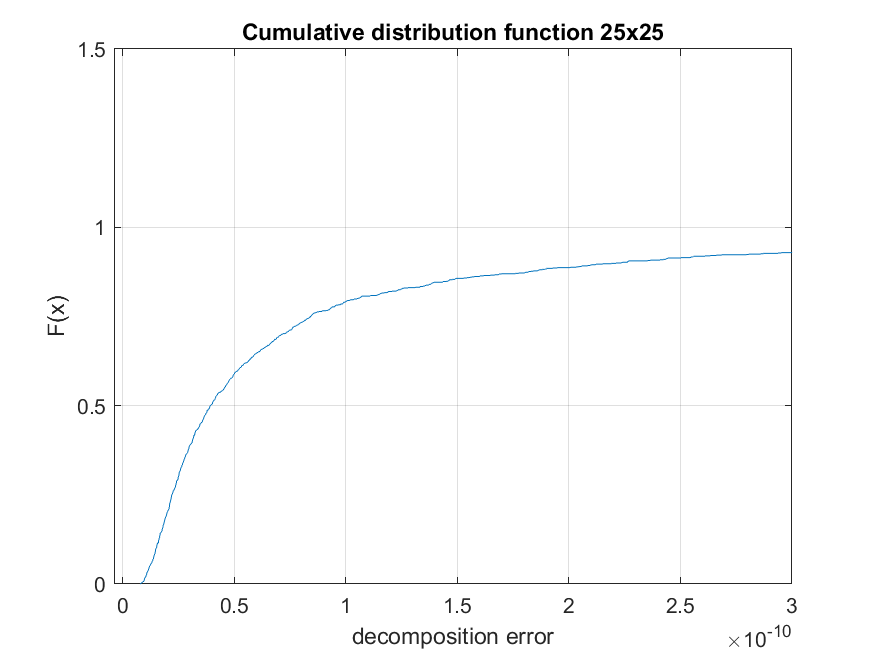
\includegraphics[scale=1]{25x25.png}
\end{center}

Wróćmy do naszej macierzy 
\begin{equation}
C =  
\begin{pmatrix}
  88.52 & 683.71 &  110,35 \\
  798.35 & 132.03 &  117.49 \\
  943 & 722.72 & 640.71 
 \end{pmatrix} 
\end{equation}
Rozwiążmy kilka równań liniowych i zobaczmy jak będzie sprawować się nasz rozkład.
Niech
\begin{equation}
    B_{1} = 
    \begin{pmatrix}
  1 & 3 &  2\\
  5 & 7 &  10 \\
  4 & 8 & 12 
  \end{pmatrix} 
  B_{2} =
  \begin{pmatrix}
  1 & 1 &  0\\
  0 & 1 &  1 \\
  0 & 0 & 1 
  \end{pmatrix}
  B_{3} =
  \begin{pmatrix}
  1 & 1 &  0\\
  0 & 1 &   \\
  0 & 0 & 1 
  \end{pmatrix}
\end{equation}
Rozwiążemy równania 
\[ LU(X1) = B_1 \] 
\[ LU(X2) = B_2 \] 
\[ LU(X3) = B_3 \] 
Otrzymujemy:

\begin{equation}
X1 =  
\begin{pmatrix}
  0.006 & 0.008 &  0.012 \\
  0.0014 & 0.004 &  0.0015 \\
  -0.005 & -0.005 & -0.0013 
 \end{pmatrix} 
\end{equation}
\begin{equation}
X2 =  
\begin{pmatrix}
  1.42 * 10^{-12} & 0.0016 &  0.0013 \\
  0.0017 & 0.0019 &  -0.00013\\
  -0.002 & -0.004 & -0.0002 
 \end{pmatrix} 
\end{equation}
\begin{equation}
X3 =  
\begin{pmatrix}
  1.42 * 10^{-6} & 0.0015 &  -0.0002 \\
  0.0017 & 0.0002 &  -0.00013\\
  -0.002 & -0.002 & 0.002 
 \end{pmatrix} 
\end{equation}
Współczynniki poprawności wynoszą kolejno:
\[ wsp_{pop}(B_1) = 8.39 * 10^{-17} \]
\[ wsp_{pop}(B_2) = 9,57 * 10^{-17} \]
\[ wsp_{pop}(B_1) = 9,18 * 10^{-17} \]
Czyli nasze równania są rozwiązane z bardzo małym błedem.
Jako że wiemy że generalnie błedy rozkładu najczęściej są bardzo małe spróbujmy sobie odpowiedzieć na jeszcze jedno pytanie. Jak rozkładają się współczynniki błędów oraz stabilności  dla macierzy, które mają mały błąd rozkładu.
Aby to zbadać wygenerowujemy 100 macierzy dla których błąd rozkładu jest różny od zera i dla każdej takiej macierzy generujemy 10 losowych układów równań. Po otrzymaniu wyników otrzymujemy:


\begin{center}
   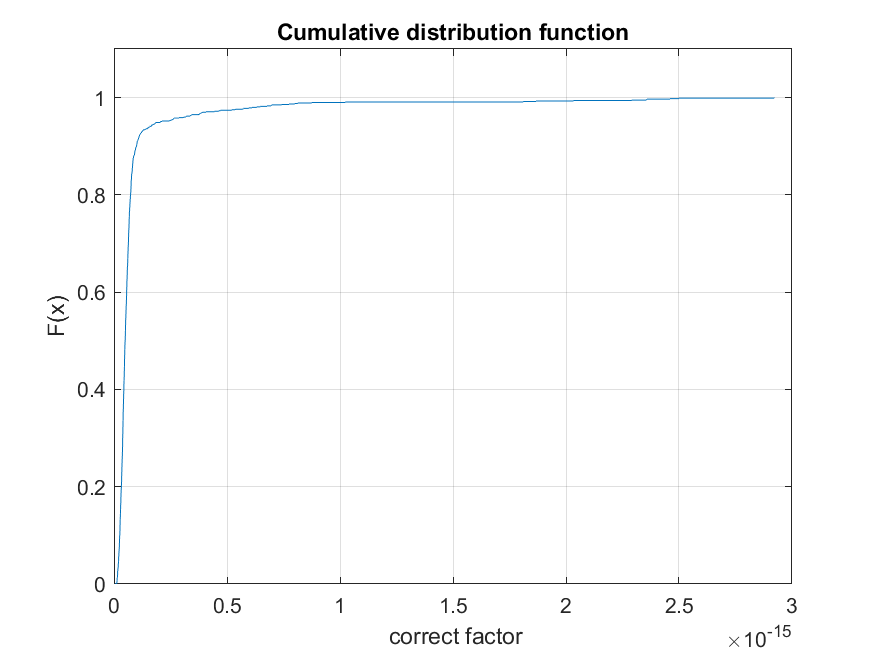
\includegraphics[scale=1]{correct_factor_cdf.png}
\end{center}
\begin{center}
   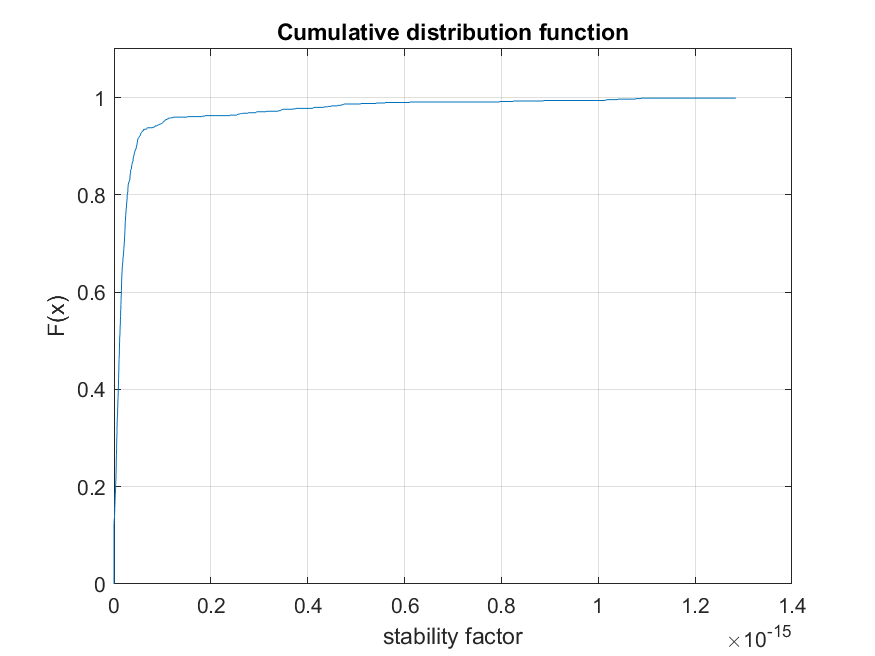
\includegraphics[scale=1]{stability_factor_cdf.png}
\end{center}

Jeśli wprowadzimy zmienne losowe: \\
Y - wynik współczynnika błędu \\
Z - wynik współczynnika stabilności
To widzimy, że 
\[P(Y < 10^{-15}) > 0.9\] 
\[P(Z < 0,2 * 10^{-15}) > 0.9\] 


 
  


\section{Analiza wyników obliczeniowych}
Powyższe przykłady pokazały nam, że wraz ze wzrostem wielkości macierzy rośnie nam ilość i wielkość błędów generowanym przez rozkład Crouta. Możemy jednak zauważyć, że przy rozmiarach $25 \times 25$ nasza macierz wciąż generuje rozkład ze względnie niewielki błędami, choć nie unikniemy błędów. Natomiast w przypadku rozkładu macierzy o niewielkich rozmiarach z całkiem wysokim prawdobodobieństwem nasza metoda wygeneruje macierz bez żadnego błędu















\end{document}
